% Test circuit
\section{Test-circuit results}\label{sec:circuit}

\subsection{Circuit and SPICE reference}
The \TestCircuit{} computes the XOR of \CircuitNumInputs{} inputs with a balanced tree of
\CircuitNumXor{} XOR2 gates. Since only the Part~B gates have leakage models, each XOR2 is built
from four NAND2 ($n_1=\overline{ab}$, $n_2=\overline{a n_1}$, $n_3=\overline{b n_1}$,
$\mathit{out}=\overline{n_2 n_3}$), giving \CircuitGateMix{} gates. All \CircuitNumVectors{}
vectors are evaluated at the same \NumCorners{} corners as the gates (\CircuitNumSims{} cases). The
SPICE reference is one flat transistor-level deck per (vector, corner), with the same subcircuits,
sizing and corners; internal nets are driven by real gates, so loading is physically present. The
output is correct in \CircuitLogicOk{} decks.

\subsection{Hierarchical ML prediction and the loading term}
A logic simulation gives every gate instance its input bits; each instance's leakage is the
Part~B ML result for that gate, input combination and corner. No SPICE quantity of the circuit is
used.

The plain gate sum under-estimated the circuit by \CircuitNoLoadBias{} (median, mean accuracy
\CircuitNoLoadMeanAcc), far more than the gate errors could explain. The missing current is
physical: in Part~B a gate's inputs are ideal sources, so the tunnelling current drawn by a high
input ($I_{in}$) is not in that gate's $I_{VDD}$. In the circuit, a high internal net is held up
by the ON PMOS of its driver, so the same current is drawn from VDD (a low net sinks into the
driver's pull-down and adds nothing). We therefore add a loading term:
\begin{equation}
  I_{VDD}^{ML} = \sum_{\text{gates}} I_{VDD}^{ML}(\text{gate},\text{bits})
  + \sum_{\text{gates}} f_{\text{int}}\, I_{in}^{ML}(\text{gate},\text{bits}),
\end{equation}
where $f_{\text{int}}$ is the share of the gate's high input pins driven by another gate (pins fed
by primary inputs draw from the testbench sources, as in the SPICE deck). On this low-power card
the term is large: it is \CircuitLoadShare{} of the predicted circuit leakage (median).

To separate the composition from the ML error, we also composed the circuit from the Part~B
\emph{SPICE} gate values with the same loading term. This reproduces the circuit SPICE leakage with
mean accuracy \CompSpiceMeanAcc{} (max error \CompSpiceMaxErr), so the hierarchical composition and
the loading term are essentially exact for this circuit, and the circuit error is inherited
entirely from the gate-level ML error.

\subsection{Results (D8)}
Over all \CircuitNumSims{} cases the mean accuracy is \CircuitMeanAcc: median error
\CircuitMedianErr, p95 \CircuitPninetyfiveErr, maximum \CircuitMaxErr, bias \CircuitBias{}
(Table~\ref{tab:circuit}, Figure~\ref{fig:circuitparity}). Grouped by the number of ones in the
vector, the accuracy stays between \CircuitOnesAccMin{} and \CircuitOnesAccMax.

\begin{table}[H]
  \centering
  \small
  \caption{Test-circuit results (D8): all vectors, then by number of ones. Below the rule: without
  the loading term, the primary-input current, and the gate-level result for comparison.}
  \label{tab:circuit}
  \fittable{% Generated by report/make_numbers.py from results/tables/circuit_results.csv. Do not edit.
\begin{tabular}{lrrrrrrrr}
\toprule
Scope & $n$ & SPICE median (A) & ML median (A) & Bias & Median err. & p95 err. & Max err. & Mean acc. \\
\midrule
all vectors & \num{51200} & \num{8.04e-10} & \num{8.11e-10} & \qty[retain-explicit-plus]{-0.16}{\percent} & \qty{0.92}{\percent} & \qty{2.91}{\percent} & \qty{5.1}{\percent} & \qty{98.92}{\percent} \\
\midrule
\quad 0 ones & \num{200} & \num{9.00e-10} & \num{9.02e-10} & \qty[retain-explicit-plus]{+0.04}{\percent} & \qty{0.87}{\percent} & \qty{2.68}{\percent} & \qty{5.1}{\percent} & \qty{98.96}{\percent} \\
\quad 1 ones & \num{1600} & \num{8.77e-10} & \num{8.75e-10} & \qty[retain-explicit-plus]{-0.03}{\percent} & \qty{0.84}{\percent} & \qty{2.73}{\percent} & \qty{5.1}{\percent} & \qty{98.96}{\percent} \\
\quad 2 ones & \num{5600} & \num{8.63e-10} & \num{8.66e-10} & \qty[retain-explicit-plus]{-0.10}{\percent} & \qty{0.88}{\percent} & \qty{2.81}{\percent} & \qty{5.1}{\percent} & \qty{98.94}{\percent} \\
\quad 3 ones & \num{11200} & \num{8.34e-10} & \num{8.39e-10} & \qty[retain-explicit-plus]{-0.14}{\percent} & \qty{0.91}{\percent} & \qty{2.88}{\percent} & \qty{5.1}{\percent} & \qty{98.93}{\percent} \\
\quad 4 ones & \num{14000} & \num{8.05e-10} & \num{8.13e-10} & \qty[retain-explicit-plus]{-0.15}{\percent} & \qty{0.93}{\percent} & \qty{2.94}{\percent} & \qty{5.0}{\percent} & \qty{98.92}{\percent} \\
\quad 5 ones & \num{11200} & \num{7.77e-10} & \num{7.84e-10} & \qty[retain-explicit-plus]{-0.20}{\percent} & \qty{0.97}{\percent} & \qty{2.97}{\percent} & \qty{5.0}{\percent} & \qty{98.91}{\percent} \\
\quad 6 ones & \num{5600} & \num{7.78e-10} & \num{7.74e-10} & \qty[retain-explicit-plus]{-0.22}{\percent} & \qty{0.98}{\percent} & \qty{2.99}{\percent} & \qty{4.9}{\percent} & \qty{98.89}{\percent} \\
\quad 7 ones & \num{1600} & \num{7.61e-10} & \num{7.66e-10} & \qty[retain-explicit-plus]{-0.21}{\percent} & \qty{0.97}{\percent} & \qty{3.04}{\percent} & \qty{4.8}{\percent} & \qty{98.89}{\percent} \\
\quad 8 ones & \num{200} & \num{7.90e-10} & \num{7.82e-10} & \qty[retain-explicit-plus]{-0.19}{\percent} & \qty{0.93}{\percent} & \qty{3.01}{\percent} & \qty{4.6}{\percent} & \qty{98.89}{\percent} \\
\midrule
without loading term & \num{51200} & \num{8.04e-10} & \num{4.82e-10} & \qty[retain-explicit-plus]{-27.59}{\percent} & \qty{27.59}{\percent} & \qty{81.70}{\percent} & \qty{96.0}{\percent} & \qty{64.79}{\percent} \\
primary-input current $I_{in}$ & \num{51200} & \num{3.43e-11} & \num{3.44e-11} & \qty[retain-explicit-plus]{-0.71}{\percent} & \qty{1.43}{\percent} & \qty{4.14}{\percent} & \qty{6.7}{\percent} & \qty{98.34}{\percent} \\
gate level (all gates) & \num{3600} & \num{2.01e-11} & \num{2.02e-11} & \qty[retain-explicit-plus]{+0.15}{\percent} & \qty{1.13}{\percent} & \qty{4.13}{\percent} & \qty{14.7}{\percent} & \qty{98.53}{\percent} \\
\bottomrule
\end{tabular}
}
\end{table}

\begin{figure}[H]
  \centering
  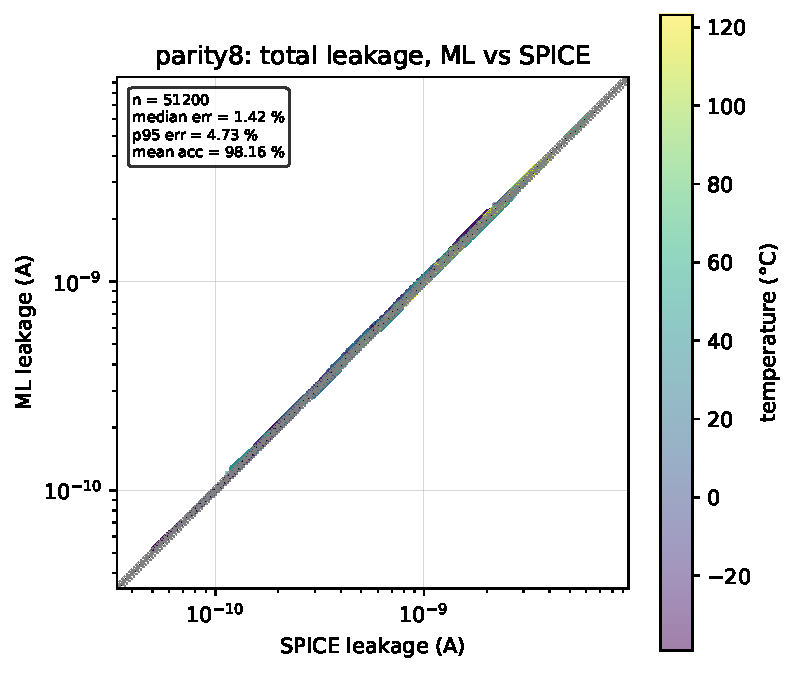
\includegraphics[width=0.6\linewidth]{circuit_parity.pdf}
  \caption{Circuit parity plot (D8), all \CircuitNumSims{} cases, coloured by temperature. The
  coldest corners sit slightly above the diagonal (Section~\ref{sec:errcircuit}).}
  \label{fig:circuitparity}
\end{figure}

\paragraph{Circuit versus gate accuracy.}
The brief expects the circuit to be less accurate than the gates. With the loading term it is
slightly \emph{more} accurate: \CircuitMeanAcc{} against \GateNandMeanAcc{} over the NAND2 cases
(its only gate type), with much smaller tails (p95 \CircuitPninetyfiveErr{} vs
\GateNandPninetyfiveErr, max \CircuitMaxErr{} vs \GateNandMaxErr). The circuit leakage is a sum
over \CircuitNumGates{} instances in different input states, so the instance-to-instance part of
the gate error partly cancels. The cancellation is incomplete because all instances share one
corner, and a systematic bias does not cancel at all: the circuit bias (\CircuitBias) stays of the
order of the NAND2 bias (\GateNandBias). The circuit accuracy is therefore limited by the
systematic part of the transistor-model error, not by its scatter.
